\documentclass[12pt,a4paper]{article}
\usepackage[utf8]{vietnam}
\usepackage{amsmath}
\usepackage{amsfonts}
\usepackage{amssymb}
\usepackage{graphicx}
\usepackage{subcaption}
\usepackage[left=2.5cm,right=2.5cm,top=2cm,bottom=2cm]{geometry}
\usepackage{listings} % môi trường để ghi code
\usepackage{color} % tô màu cho code
\usepackage{blindtext}
\usepackage[unicode]{hyperref}
% ------------------------ Giúp khởi tạo môi trường viết code (tự động tô màu Syntax)
\definecolor{dkgreen}{rgb}{0,0.6,0}
\definecolor{gray}{rgb}{0.5,0.5,0.5}
\definecolor{mauve}{rgb}{0.58,0,0.82}
\lstset{frame=tb,
  language=C,
  aboveskip=3mm,
  belowskip=3mm,
  showstringspaces=false,
  columns=flexible,
  basicstyle={\small\ttfamily},
  numbers=none,
  numberstyle=\tiny\color{gray},
  keywordstyle=\color{blue},
  commentstyle=\color{dkgreen},
  stringstyle=\color{mauve},
  breaklines=true,
  breakatwhitespace=true,
  tabsize=3
}
%----------------------------
\renewcommand{\baselinestretch}{1.3} % lệnh này cho phép điều chỉnh khoảng cách chung giữa CÁC DÒNG
\setlength{\parskip}{0.3em} % Lệnh này điều chỉnh khoảng cách giữa CÁC ĐOẠN

\title{\textbf{ ỨNG DỤNG THUẬT TOÁN PHÂN CỤM K-MEANS TRONG NÉN ẢNH   }\thanks{Bài tiểu luận giới thiệu về phương pháp phân cụm cơ bản áp dụng trong nén hình ảnh và sơ qua các phương pháp cải tiến thuật toán này.}}
\date{2020\\ July}
\author{Phạm Anh Tuấn, Đỗ Thị Tâm Linh An \\ \\ \textit{Posts and Telecommunications Institute of Technology,} \\ \textit{Km10, Đường Nguyễn Trãi, Q.Hà Đông, Hà Nội}}

\begin{document}
\maketitle
\begin{center}
	\textbf{\large Tóm Tắt}
\end{center}


Được cho là sự kết hợp của văn bản, âm thanh hay hình ảnh đặt trong môi trường số - Đa Phương Tiện được biết đến như một đại lượng thông tin mà dữ liệu được biểu diễn dưới dạng "Kép". Việc tối ưu hoá không gian lưu trữ dữ liệu mà chất lượng không bị giảm nhiều là điều cần thiết. Bên cạnh việc cải tiến các hệ thống giao thức truyền thông, thì việc nén dữ liệu cũng quang trọng không kém. Tôi ưu hoá dữ liệu củng cố rất nhiều hiệu quả trong khả năng truyền tải, xử lý thông tin giữa các mạng lưới thiết bị trong thời đại số hiện nay. Trong khuôn khổ  báo cáo này chúng ta chỉ xét đến việc nén hình ảnh trong phân ngành xử lý hình ảnh, cụ thể bằng việc sử dụng hoc máy trong việc nâng cao hiệu quả nén ảnh.
\newpage
\section{Giới thiệu }

Việc xử lý ảnh nói chung hay nén ảnh nói riêng luôn được chú trọng quan tâm và cải thiện từ khi xuất hiện lần đầu cho đến nay. Trong khoảng thời gian đó đã có rất nhiều phương pháp nén ảnh tôi ưu từ nén không tổn hao và nén tổn hao. Ở nén tổn hao thì các phương pháp đa dạng hơn có thể kể đến: Nén cơ bản (\textit{Baseline Sequential Mode}), nén luỹ tiến (P\textit{rogressive Mode}) và nén phân cấp (\textit{Hierarchical Mode}). Các phương pháp này chỉ khác nhau trong phương thức ta mã hoá các hệ số \textbf{DCT}.

Sơ lược về cách hoạt động của thuật toán \textbf{DCT} (Biến đổi cosin rời rạc) là dựa vào các đặc tính của thị giác con người để loại bỏ bớt thông tin "Dư thừa" có trong một bức ảnh. Ý tưởng của phép biến đổi này bắt đầu bằng việc chia bức ảnh nhiều ô vuông nhỏ và biểu diễn nó dưới dạng ma trận. Trị số lớn ta biểu diễn cho cường độ Pixel lớn và ngược lại đối với trị số nhỏ trong ma trận.

\begin{center}
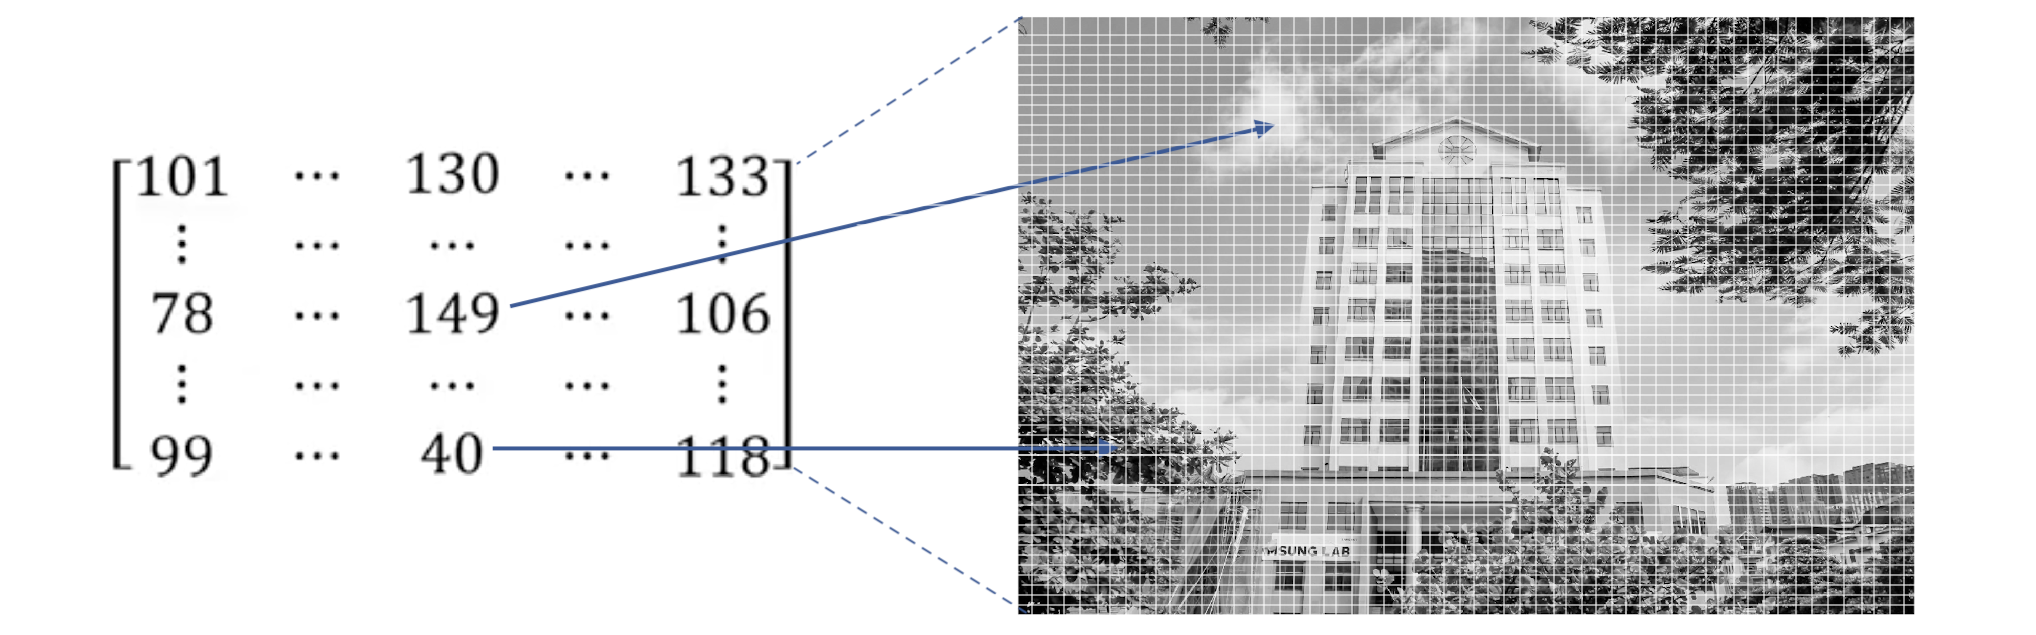
\includegraphics[scale=0.45]{Bieudienbinary.png}
\end{center}

Hình ảnh kỹ thuật số ngày nay thường lưu dưới các kênh màu RGB. Tuy nhiên trong nén ảnh chúng ta lại sử dụng một kênh màu khác. Như đã đề cập ở trên, nén ảnh tổn hao chú trọng vào việc loại bỏ thông tin dư thừa mà ta không dễ nhận thấy trong một bức ảnh. Chính vì vậy hệ YCbCr được sinh ra để thay thế. Với kênh Y để biểu diễn cường độ ánh sáng và 2 kênh còn lại là Cb và Cr.

\begin{center}
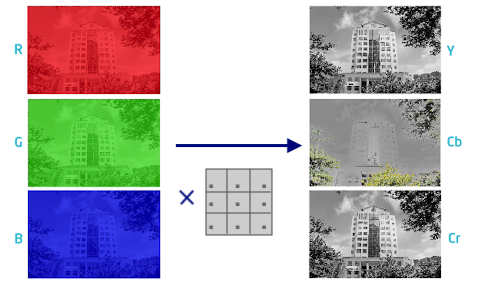
\includegraphics[scale=0.65]{ColorSpaceConversion.png}
\end{center}

Tiếp sau khi chuyển đổi không gian màu của bức ảnh, ta sẽ dựa vào đặc điểm thị giác con người để điều chỉnh thích hợp các kênh màu để giảm lượng lưu trữ nhưng đảm bảo lượng thông tin trong bức ảnh. Cụ thể, các kênh màu như \textbf{Cb} và \textbf{Cr} sẽ được giảm xuống so với kênh \textbf{Y} do mắt chúng ta nhạy cảm với thay đổi ánh sáng so với màu sắc. Bên cạnh đó khả năng nhận biết thông tin có trong bức ảnh còn phụ thuộc vào tương quan độ tương phản và tần số, được biểu diễn qua biểu đồ dưới đây. Như hình \textbf{b)} bên dưới, phần thông tin hình ảnh với tần số cao và độ tương phản thấp khầu như không nhận thấy được phần không gian dưới đường kẻ trắng. Đồng nghĩa với việc những khu vực trên ngoài đường kẻ trắng sẽ được tập trung nén.
\begin{center}
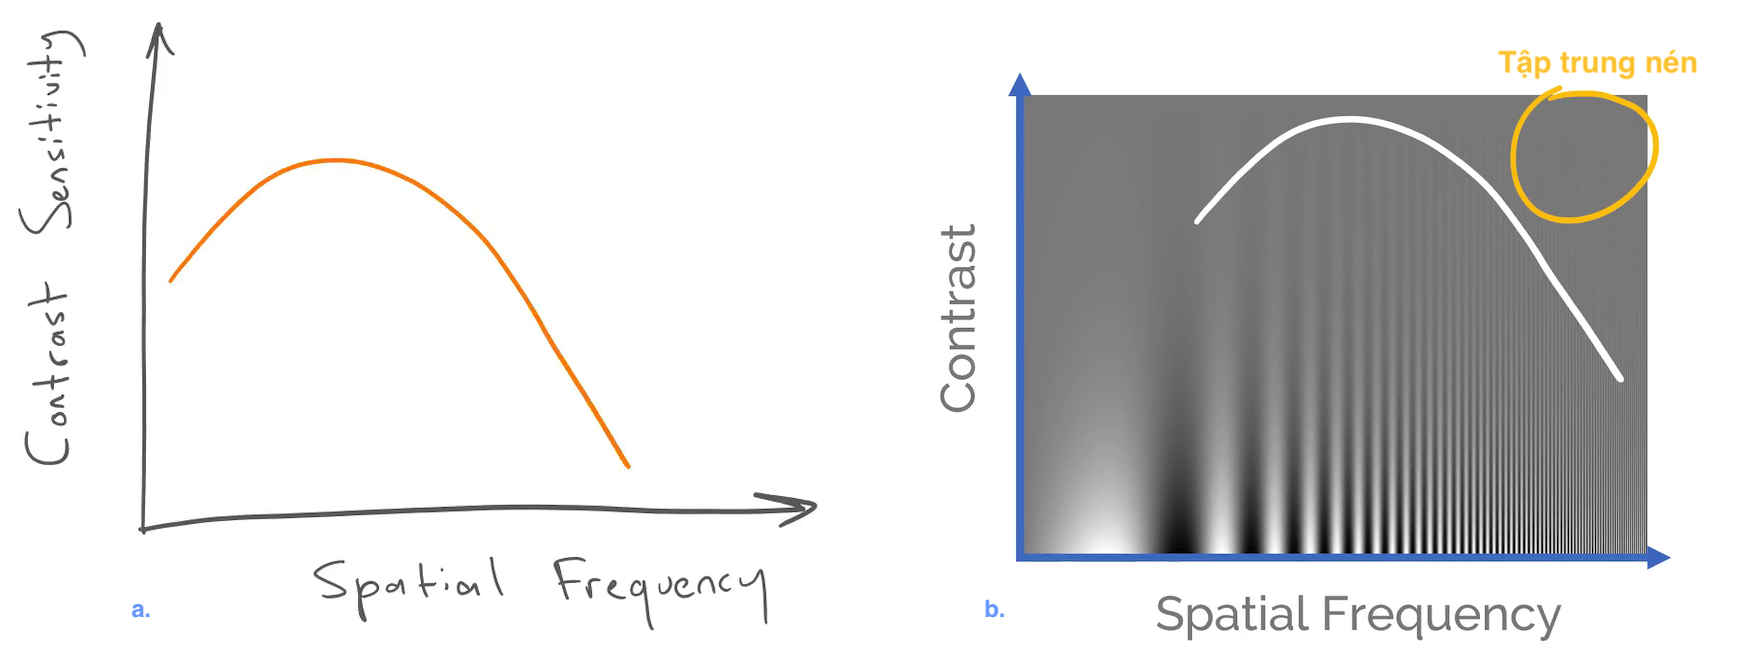
\includegraphics[scale=0.25]{frequencyandcontrast.png}
\end{center}

Vậy DCT đã làm gì? Đó là chia hình ảnh thành các khối 8*8 và lượng tử hoá chúng thành các đại diện cho miền tần số. Rõ ràng hơn, bằng việc so sách từ khối vuông 8x8 với 64 mẫu tần số với sự tăng dần tần số từ trái sang phải và từ trên xuống dưới như hình.
\begin{center}
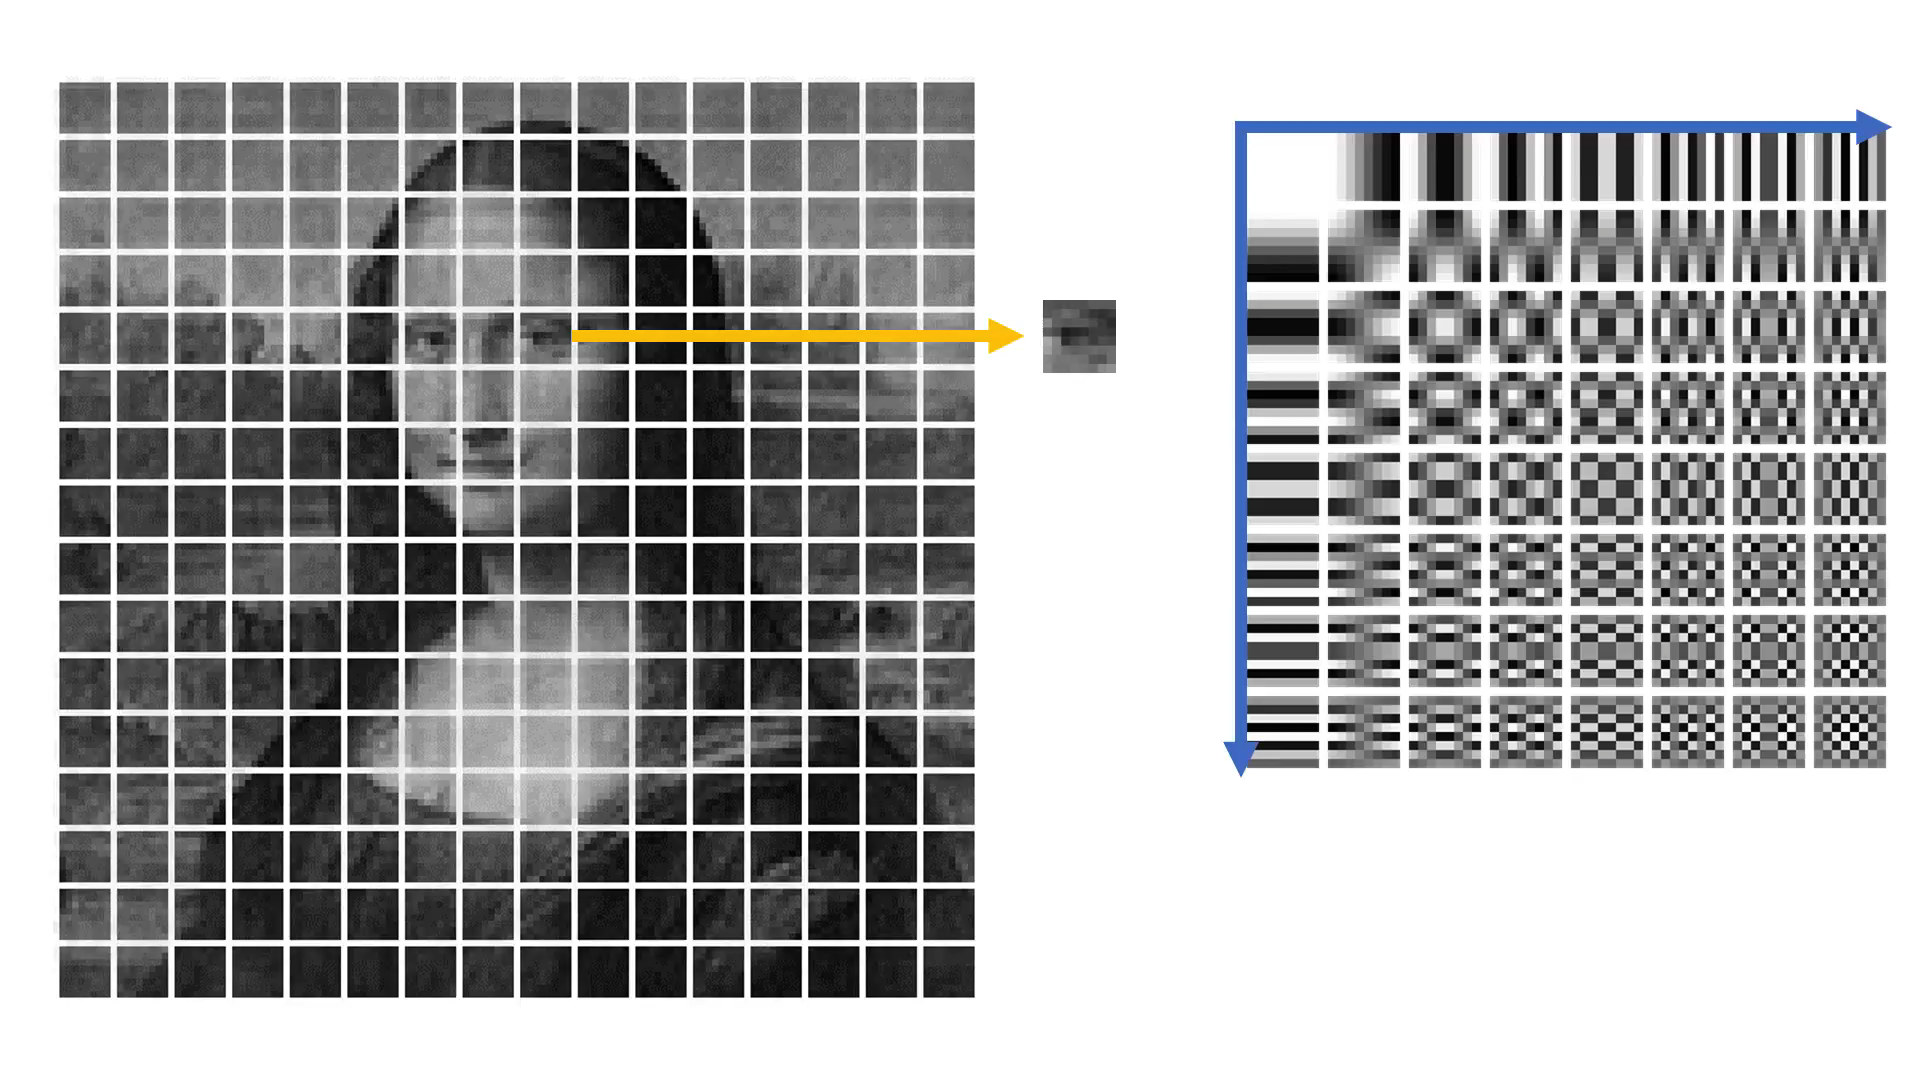
\includegraphics[scale=0.25]{Quantumize.png}
\end{center}

Chúng ta sẽ sử dụng phương trình $(1)$ cho việc biến đổi các lưới ô 8*8 sử dụng biểu đồ bước sóng như hình phía trên. Quá trình tương tự biến đổi Fourier hai chiều, sự khác biệt là sử dụng hàm Cosin và hàm Gamma:
$$\mathbf{F(u,v)} = (\dfrac{2}{N})^{\frac{1}{2}} (\dfrac{2}{M})^{\frac{1}{2}} \sum_{i=0}^{N-1}\sum_{j=0}^{M-1} (\wedge{(i)}\wedge{(j)} \left[ \cos{\left(\dfrac{u\cdot\pi}{2N}(2i+1)} \right) \cos{\left(\dfrac{u\cdot\pi}{2M}(2j+1)} \right) \right] $$
$$$$

Sau cùng, với ma trận biểu thị độ nhạy cường độ Pixel ta biểu diễn thành một khối tương tự mà đơn vị ma trận lại biểu diễn một thành phần tần số cụ thể. Phương pháp này là phương pháp biến đổi Cosin rời rạc
\begin{center}
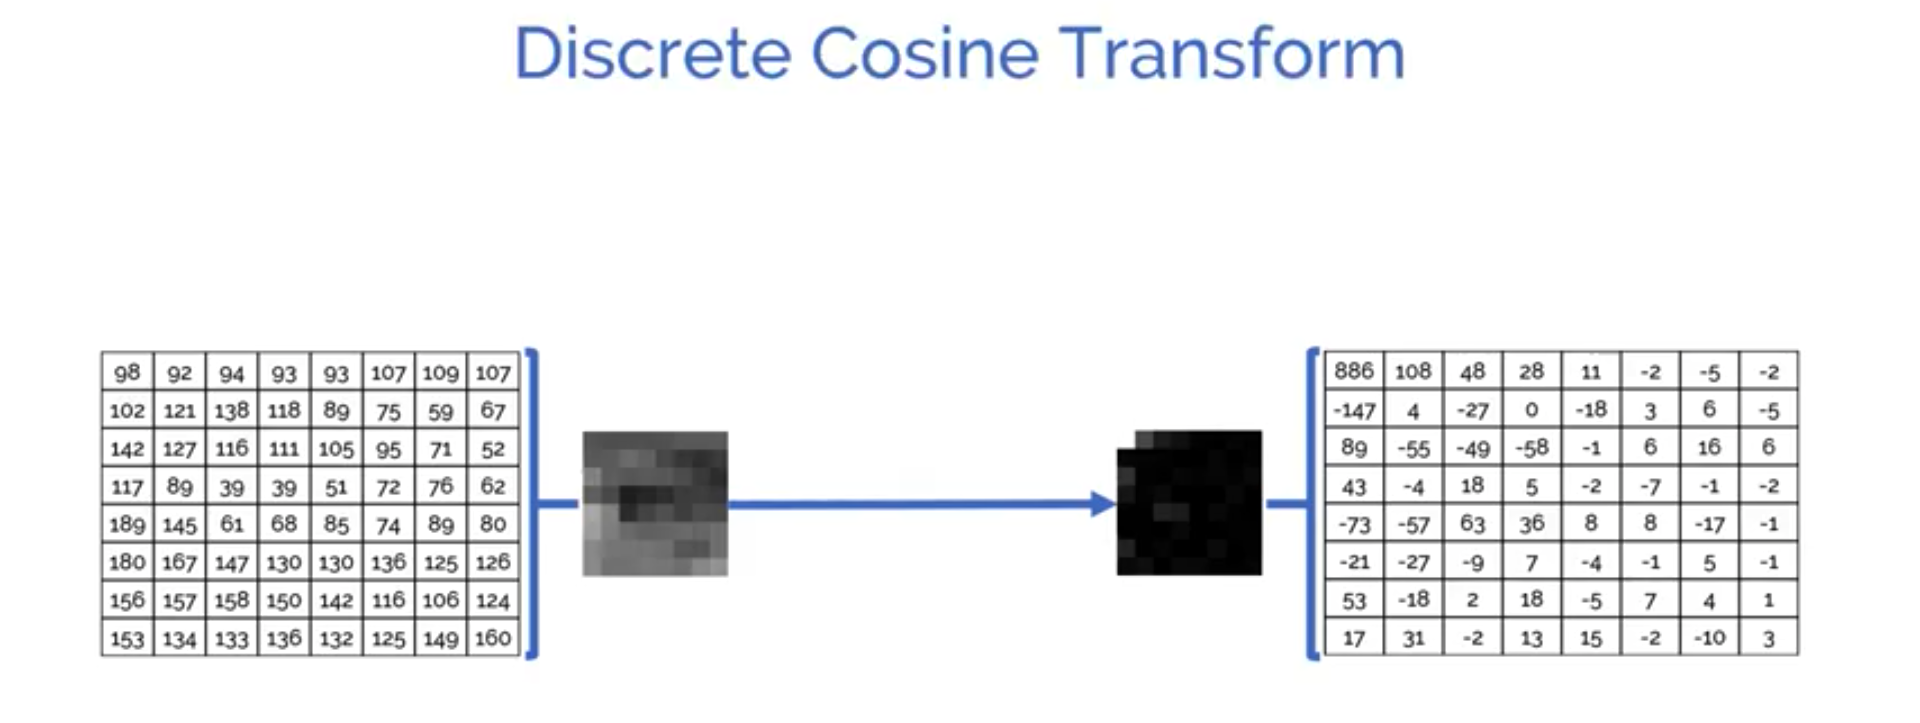
\includegraphics[scale=0.25]{DiscreteCosineTransform.png}
\end{center}

Bản thân DCT không nén hình ảnh mà cung cấp thông tin bản chất của quá trình nén - thứ thật sự diễn ra sau quá trình biến đổi Cosin rời rạc (DCT). Sơ qua toàn bộ quá trình để có một bức ảnh nén hoàn chỉnh sẽ được biểu diễn ở hình bên dưới:
\begin{center}
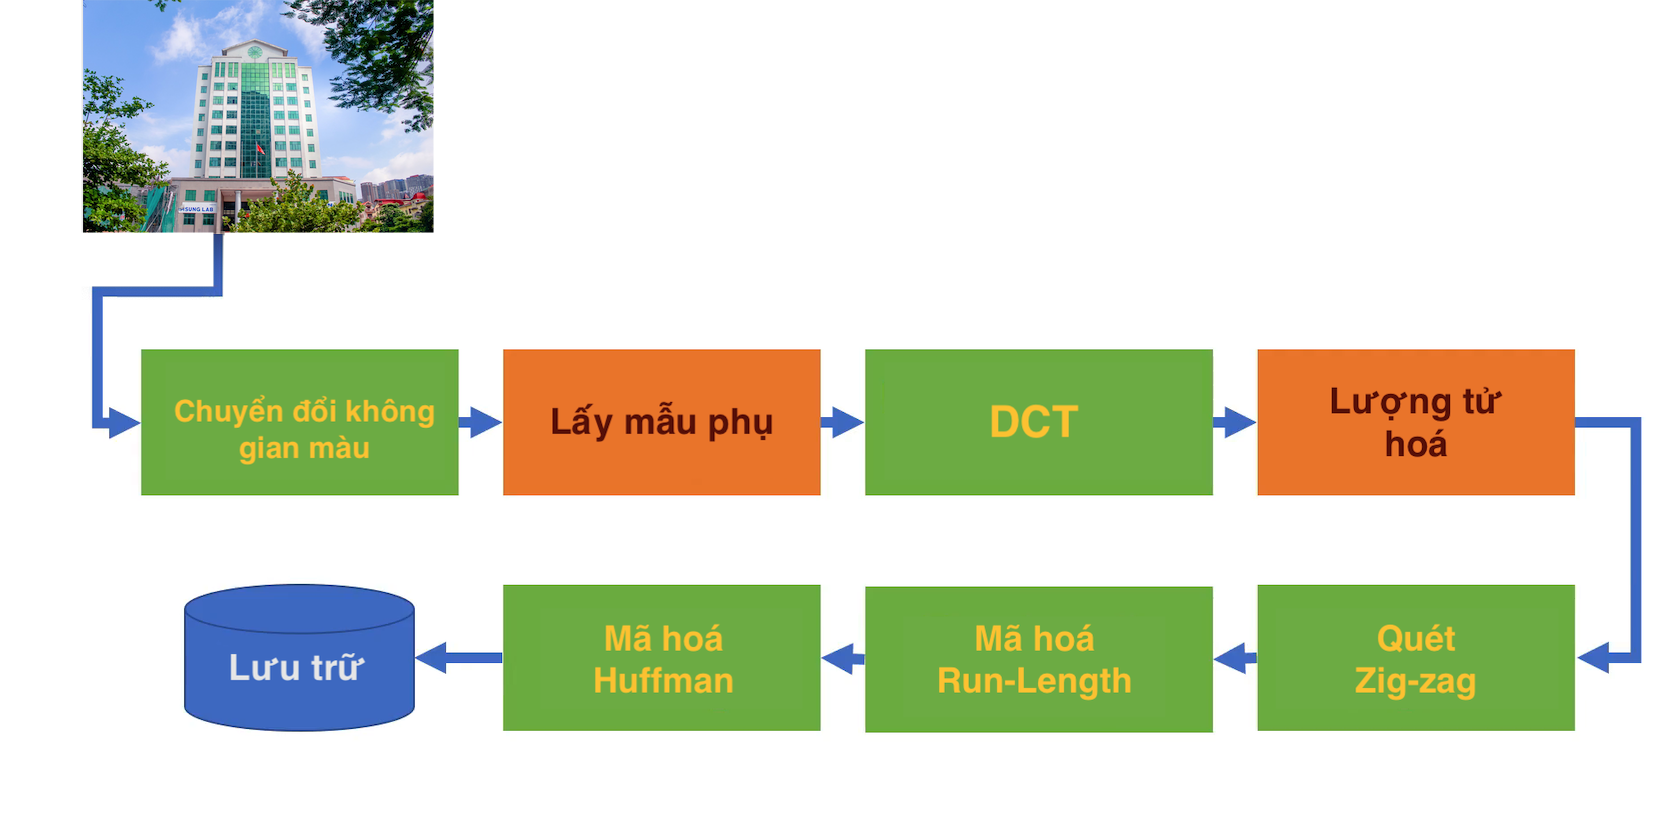
\includegraphics[scale=0.25]{imagecompressprocess.png}
\end{center}
\newpage
\section{Đề xuất và phân tích thuật toán K-Means }
\subsection{Ý tưởng}

Quay trở lại với phương pháp nén ảnh bằng phân cụm K-Means. Phương pháp này có những ưu điểm vượt trội như khả năng hoạt động đơn giản của thuật toán (giữ nguyên kênh màu RGB mà không cần chuyển đổi kênh màu như kỹ thuật cũ, không cần công đoạn chuyển đổi tần số v.v ...), xử lý hiệu quả với bộ dữ liệu lớn,...  Đây là một thuật toán không quá mới trong khoa học máy tính và đặc biệt là học máy. Ý tưởng của thuật toán này là việc phân chia một bộ dữ liệu thành các cụm khác nhau mà các thành viên trong cụm đó chung hay có những đặc điểm tương đông. Việc phân cụm sẽ được diễn ra tự động với số lần lặp để xác định chính xác điểm tụ của mỗi cụm \footnote{Điểm tụ là điểm xác định trung tâm của cụm dữ liệu đó. }. Trong nén ảnh, ta sẽ coi dữ liệu là các điểm trong không gian, các điểm dữ liệu này càng gần nhau thì càng giống .
\begin{center}
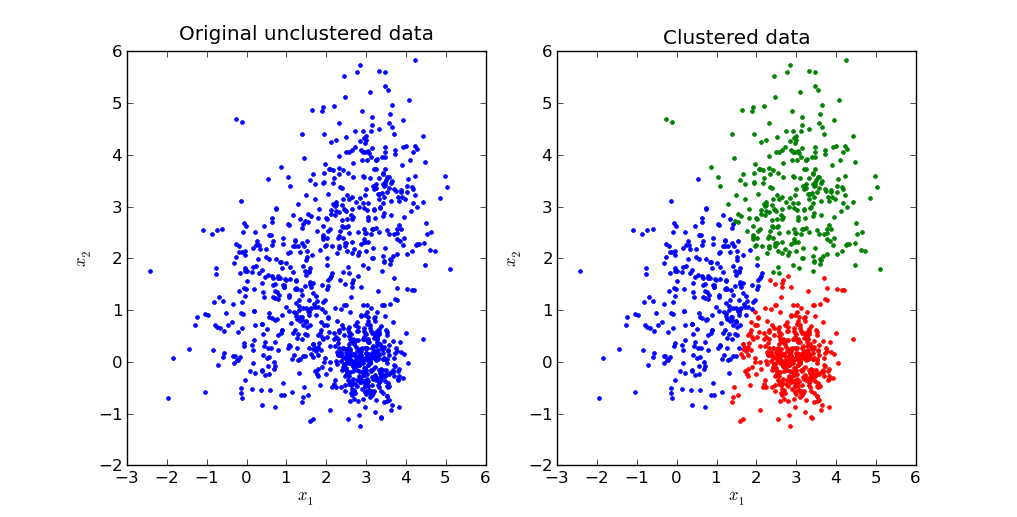
\includegraphics[scale=0.45]{kmean1.png}
\end{center}

Từ ý tưởng và nguyên lý làm việc của thuật toán, ta đưa ra một mô hình toán học bắt đầu bằng việc đặt một đầu vào dữ liệu $X \in R^{nd}$ trong đó $N$ là số điểm dữ liệu và $d$ là chiều cho từng mẫu dữ liệu đó. Thuật toán sẽ có nhiệm vụ chính là chia $N$ dữ liệu đó thành $K$ cụm (thoả mãn $K$\leq $N$ )~ $ mà các dữ liệu trong mỗi cụm là giống nhau. Đầu ra của thuật toán là xác định và xuất ra trung tâm (center) hoặc nhãn (label) của cụm dữ liệu đó. $

\subsection{Giải thuật}
Giả sử chúng ta có $\textit{N}$ điểm dữ liệu là $\mathbf{X} = [\mathbf{x}_1, \mathbf{x}_2, \dots, \mathbf{x}_N] \in \mathbb{R}^{d \times N}$ và thuật toán bắt đầu bằng việc khởi tạo $k$ điểm bất kì làm điểm trung tâm của Cluster (cụm dữ liệu)
\begin{align}
$$\mathbb{C}^{(0)}=\{m_1^{(0)},m_2^{(0)}, ... ,m_k^{(0)}\}$$
\end{align}

Giá trị sau khỉ khởi tạo sẽ tiến đến quá trình nhóm dữ liệu, ở bước này 
các điểm dữ liệu sẽ được nhóm đến các cụm dữ liệu có trung tâm gần nhất với nó :
\begin{align}
$$\mathbb{S}_i^{(t)}=\{x_p:\Vert{x_p-m_i^{(t)}}\Vert^2 \le \Vert{x_p-m_j^{(t)}}\Vert^2\} ~~~,\forall j,1 \le j \le k$$
\end{align}

Các tâm cụm sẽ được cập nhật lại bằng cách lấy trung bình cộng khoảng cách tới các điểm dữ liệu và sẽ lặp lại qua phương trình 2 cho đến khi các cụm của các nhóm không thay đổi thêm thì dừng giải thuật:
\begin{align}
$$m_i^{(t+1)}=\frac{1}{\vert{\mathbb{S}_i^{(t)}}\vert} \sum_{x_j\in\mathbb{S}_i^{(t)}}x_j$$
\end{align}

Lưu đồ biểu diễn của thuật toán được biểu diễn như hình dưới
\begin{center}
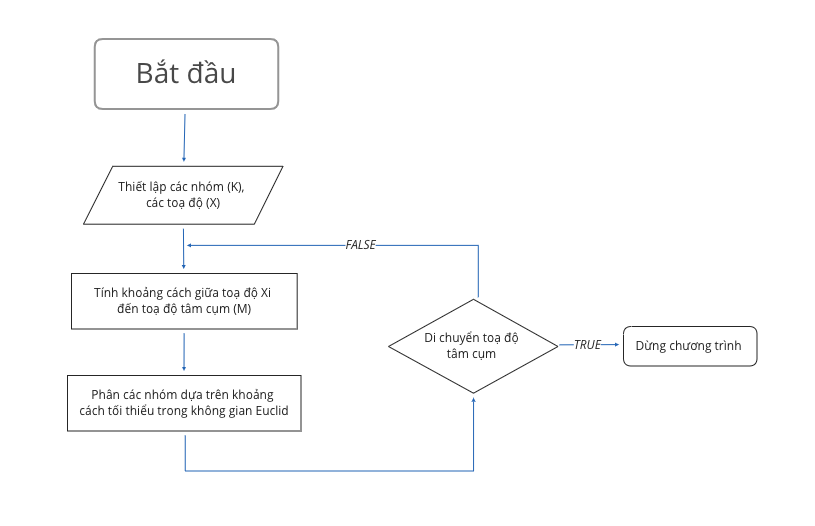
\includegraphics[scale=0.55]{flowchartkmeans.png}
\end{center}

\subsection{Hàm mất mát và bài toán tối ưu}
Trước khi đi sâu vào bài toán, với mỗi điểm $\mathbf{x}_i$ nếu được phân vào một cụm $\mathbf{k}$ ta đặt $\mathbf{y}_i = [\mathbf{y}_{i1}, \mathbf{y}_{i2}, \dots, \mathbf{y}_{iK}] $ là Label Vector của nó. Khi đó $\mathbf{y}_{jk} = 1$ và $y_{ij} = 0, \forall j \neq k$ từ đó dẫn tới phương trình ràng buộc của $y_{i}$ như sau: 
\begin{align}
$$y_{ik} \in \{0, 1\},~~~ \sum_{k = 1}^K y_{ik} = 1 $$
\end{align}

Khi đó, nếu ta coi $m_{k}$ là tâm mỗi cụm và các điểm để xác định được phân vào một cụm (Cluster) được xác định bởi $m_{k}$. Khi đó sai số của một điểm dữ liệu $x_{i}$ khi phân vào cụm sẽ là $(x_{i} - m_{k})$. Như mục tiêu ban đầu của thuật toán là khiến trị tuyệt đối của sai số này nhỏ nhất: 
\begin{align}
$$\|\mathbf{x}_i - \mathbf{m}_k\|^2 \rightarrow Min$$ 
\end{align}

Theo phương trình $(4)$ trước đó, biểu thức $(5)$ được viết lại thành: 
\begin{align}
$$y_{ik}\|\mathbf{x}_i - \mathbf{m}_k\|^2 =  \sum_{j=1}^K y_{ij}\|\mathbf{x}_i - \mathbf{m}_j\|^2$$
\end{align}

Với $\mathbf{Y} = [\mathbf{y}_1; \mathbf{y}_2; \dots; \mathbf{y}_N]$, $\mathbf{M} = [\mathbf{m}_1, \mathbf{m}_2, \dots \mathbf{m}_K]$ lần lượt là các ma trận Label Vector và tâm cụm. Bài toán ta cần tối ưu quay trở về dạng sau, ($argmin$ là điều kiện giá trị của biến số để hàm số đang xét đạt giá trị nhỏ nhất): 
\begin{align}
$$\mathbf{Y}, \mathbf{M} = \arg\min_{\mathbf{Y}, \mathbf{M}} \sum_{i=1}^N\sum_{j=1}^K y_{ij} \|\mathbf{x}_i - \mathbf{m}_j\|^2$$ 
\end{align}

\subsection{Thuật toán tối ưu hàm mất mát}
Ở phương trình $(7)$ rất khó để tìm điểm tối ưu hay chính xác là việc tìm nghiệm tối ưu toàn cục (global optimal point) do có thêm các điều kiện ràng buộc. Bài toán trước mắt ta sẽ tập trung vào phương pháp tìm điểm gần đúng hay điểm cực tiểu. $\mathbf{Y}$ và $\mathbf{M}$ là 2 biến có thể thay đổi được và được tận dụng để xử lý bài toán này  
\subsubsection{Cố định M, tâm của cụm}
Giả sử các Centers đã được biết hoặc cho trước, khi đó cần tìm các Label Vector để hàm mất mát đạt giá trị cực tiểu. Khi các Centers là cố định, phương trình $(7)$ được rút gọn lại thành:
\begin{align}
$$\mathbf{y}_i = \arg\min_{\mathbf{y}_i} \sum_{j=1}^K y_{ij}\|\mathbf{x}_i - \mathbf{m}_j\|^2 $$
\end{align}

Ta biết chỉ một phần tử của Label Vector $y_{i}$ bằng 1 nên phương trình $(8)$ có thể tiếp tục viết lại dưới dạng 
\begin{align}
$$j = \arg\min_{j} \|\mathbf{x}_i - \mathbf{m}_j\|_2^2$$
\end{align}

Từ $(9)$ ta nhận thấy $\|\mathbf{x}_i - \mathbf{m}_j\|^2$ chính là bình phương khoảng cách từ $\mathbf{x}_i$ tới Center $\mathbf{m}_j$. Rút ra kết luận: \textbf{Mỗi điểm $\mathbf{x}_i$ thuộc về Cụm có Tâm gần đó nhất. }
\subsubsection{Cố định Y, Label Vector}
Giả sử Label Vector được cố định, phương trình $(7)$ được rút gọn thành
\begin{align}
$$\mathbf{m}_j = \arg\min_{\mathbf{m}_j} \sum_{i = 1}^{N} y_{ij}\|\mathbf{x}_i - \mathbf{m}_j \|^2$$ 
\end{align}

Nhận thấy rằng phương trình $(10)$ là một hàm lồi và khả dĩ trên đoạn $i \in [1, N]$ nghiệm của phương trình có được bằng phương pháp giải đạo hàm bằng $0$ 

Đặt $l(\mathbf{m}_j)$ thay cho $\arg\min$, ta có đạo hàm cho phương trình $(10)$ như sau: 
\begin{align}
$$\frac{\partial l(\mathbf{m}_j)}{\partial \mathbf{m}_j} = 2\sum_{i=1}^N y_{ij}(\mathbf{m}_j - \mathbf{x}_i)$$
\end{align}

Giải phương trình với đạo hàm bằng $(0)$ ta được:
\begin{align}
$$\mathbf{m}_j \sum_{i=1}^N y_{ij} = \sum_{i=1}^N y_{ij} \mathbf{x}_i$$
$$\Rightarrow \mathbf{m}_j = \frac{ \sum_{i=1}^N y_{ij} \mathbf{x}_i}{\sum_{i=1}^N y_{ij}}$$
\end{align}

Điểm đặc biệt của phương trình $(12)$ đó là mẫu số chính là phép đếm số lượng các điểm dữ liệu có trong \textbf{Cluster} $j$ còn tử số là tổng các điểm dữ liệu có trong \textbf{Cluster} $j$. Rút ra kết luận một cách tổng quan rằng: $\mathbf{m}_j$ chính là trung bình cộng các điểm trong \textbf{Cluster} $j$

\section{Chương trình và tính hiệu quả (not done yet)}
Bằng việc đưa thuật toán về K-Means vào trong ứng dụng viết bởi C++, đã đưa ra dữ liệu về tính hiệu quả cũng như khả năng của thuật toán này. Do mỗi bức ảnh chứa 3 không gian màu, đã thu được kết quả sau 

\section{Nhận định và cải tiến thuật toán}
\subsection{Nhận định}
Từ kết quả của chương trình, cũng như qua biểu diễn toán học của thuật toán, dễ dàng nhận thấy những đặc điểm nổi bật của thuật toán này cũng chính là yếu điểm của nó. Cụ thể các ảnh khi được xử lý rất đơn giản và nhanh chóng được thực hiện, tuy nhiên tốc độ xử lý của thuật toán sẽ trở nên chậm chạp và sẽ không phù hợp với một tập dữ liệu cũng như cụm phức tạp. Độ hội tụ của tâm cụm sẽ chậm đi khi xử lý một bức ảnh lớn (nhất là những bức ảnh thiên văn học). Ngoài ra, do ở bước đầu trong việc triển khai thuật toán, tâm cụm được khởi tạo ngẫu nhiên, chính vì vậy nếu các cụm được tạo "không tốt" như quá gần nhau ... thì việc xác định các tâm cụm hội tụ về đúng điểm lả rất lâu là đôi khi có thể gây lỗi cho chương trình. Và các nhà khoa học đang không ngừng cải thiện làm sao cho tâm cụm được khởi tạo tốt nhất.

\subsection{Cải tiến}
Qua phần nhận định trên, chúng ta đã thấy việc xác định các tâm cụm (mặc dù là ngẫu nhiên) ảnh hưởng rất nhiều đến hiệu quả của thuật toán. Chính vì vậy thuật toán cải tiến dưới đây - wiKmeans áp dụng phép biến đổi Wavelet sẽ tập trung vào cải thiện phân vùng ảnh. Lưu đồ thuật toán của wiKmeans được biểu diễn như hình dưới:

\begin{center}
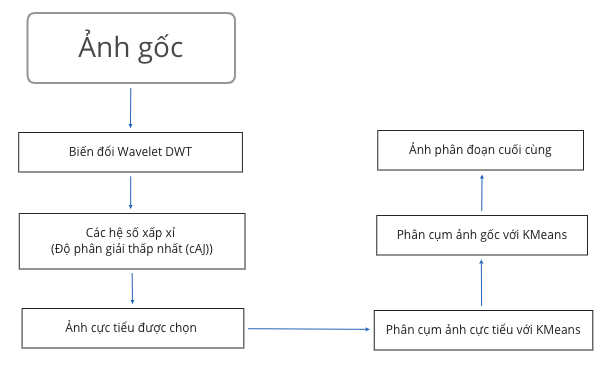
\includegraphics[scale=0.6]{wikmeans.png}
\end{center}

\subsubsection{Biến đổi wavelet}
Ở bước này, phép biến đổi wavelet được dùng giàm kích thước ảnh. Sau khi thực hiện phép biến ta thu được hệ số \textit{wavelet} là hàm co giãn và vị trí của sóng nhỏ. Biến đổi sóng nhỏ có thể được biểu diễn tương tự như biến đổi \textit{Fourier}:$$\mathbf{F(w)} = \int_{-\infty}^\infty f(t) \mathbf{e}^{jwt} \;\mathrm{d}t $$
$$\mathbf{C}(scale,position) = \int_{-\infty}^\infty s(t) \omega (scale,position,t) \;\mathrm{d}t $$

Tập hệ số Wavelet có thể thu được nhờ phép biến đổi sóng nhỏ rời rạc (Discrete Wavelet Transform - DWT). Với phần lớn ảnh số thì nội dung tần số thấp là quan trọng nhất, giữ được hầu như các đặc tính của ảnh đầu vào của phép biến đầu với kích thước giảm bốn lần. Sau khi áp dụng bộ lọc thông thấp theo hai hướng (LL) ta thu được ảnh xấp xỉ (cA1) của ảnh gốc. Nếu áp dụng bộ lọc thông thấp cho chiều ngang và bộ lọc thông cao cho chiều dọc ảnh (LH) ta có tập hệ số ngang (cH1) của ảnh gốc. Tương tự ta có tập hệ số dọc (cV1) và tập hệ số chéo (cD1). Lặp tiến trình trên băng con (LL) để sinh ra các hệ số ở mức 2 tiếp theo. Hình 2 mô tả DWT ảnh theo thuật toán hình kim tự tháp của Mallat [4].

\begin{center}
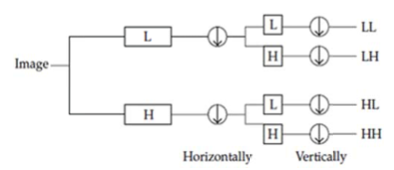
\includegraphics[scale=0.7]{biendoianhwave.png}
\end{center}

Vậy ảnh gốc S được biểu diễn trên cơ sở các hệ số biến đố sóng con của nó như sau: $$\mathbf{S} = cA_1 + \{cH_1 + cV_1 + cD_1\}$$

Thực hiện lặp tiến trình cho đến khi mức độ chi tiết là mẫu hay pixel. Tại mức J, ảnh gốc được biểu diễn bởi: $$\mathbf{S} = cA_J + \{cH_i + cV_i + cD_i\}_{j=1}^J$$

Các hệ số xấp xỉ được tính toán như sau: $$\mathbf{cA}_{j-1} = cA_J + \{cH_j + cV_j + cD_j\}$$

Mỗi lần thực hiện phân rã wavelet, kích thước của ảnh xấp xỉ cAj giảm đi bốn lần so với lần thực hiện trước đó (mỗi chiều giảm xuống một nửa). Như vậy, giả sử chúng ta phân rã 3 mức cho ảnh đầu vào, ta thu được ảnh xấp xỉ có kích thước giảm xuống 64 lần.

\subsubsection{Phân cụm Kmeans ảnh cực tiểu}
Tiến hành phân cụm ảnh xấp xỉ cực tiểu lựa chọn với thuật toán KMeans. Sau khi đã phân cụm tất cả các ô, ta được tập tâm cụm như sau:$$\mathbf{V}_{Init} = \{ \mathbf{v}_k; 1\leq k\leq c \}$$

\subsubsection{Phân cụm Kmeans theo ảnh gốc}
Thực hiện phân việc phân cụm ảnh gốc với thuật toán KMeans với tập tâm cụm khởi tạo VInit thu được trong B2.

\subsubsection{Thử nghiệm và kết quả}
Bằng việc áp dụng thuật toán đề xuất wiKMeans và so sánh kết quả với thuật toán Kmeans trước đó. Bảng sau đây cho thấy thời gian phân cụm của một bức ảnh trong hai thuật toán trong trường hợp số cụm bằng 5

\begin{center}
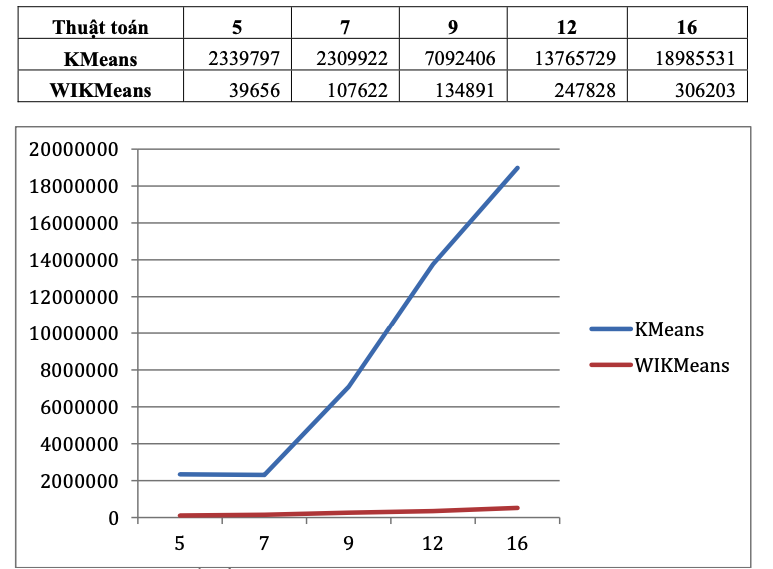
\includegraphics[scale=0.5]{kmeansimprovedata.png}
\end{center}

Bảng sau đây đưa ra số liệu về khoảng cách các tâm cụm của thuật toán wiKMeans và KMeans trong trường hợp 5 cụm 

\begin{center}
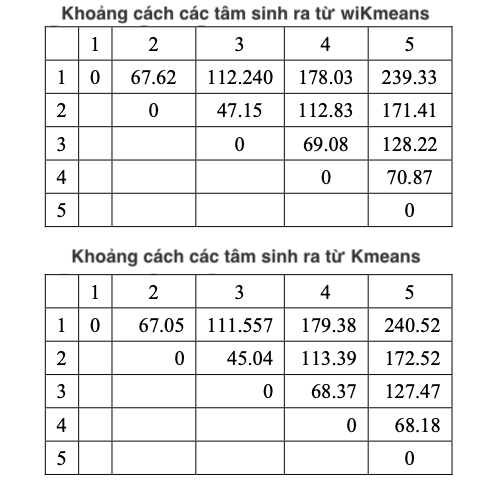
\includegraphics[scale=0.5]{kmeansimprovedata2.png}
\end{center}

\section{Kết luận}
Kmeans là một thuật toán đơn giản với nhiều ưu điểm cải tiến so với các thuật toán nén ảnh thuần tuý trước đó. Mặc dù vậy các nhược điểm của thuật toán như khởi tạo tâm cụm hay xử lý điểm tụ là điều rõ ràng. Đã có rất nhiều thuật toán dựa trên Kmeans nhưng được cải thiện về các nhược điểm có thể kể Đến Kmeans++ ,K-SVD.. Tuy nhiên trong khuôn khổ bài báo cáo ta chỉ xét qua về ý tưởng ban đầu về thuật toán Kmeans và qua đó điểm qua việc sử dụng biến đổi wavelet để cải thiện thuật toán. 

\section{Tài liệu tham khảo}

\end{document}


